\chapter{IoT}
Il progetto eServant include al suo interno due principali tecnologie che rientrano nella categoria
"Internet Of Things":
\begin{itemize}
    \item dispositivi BLE per geolocalizzare i partecipanti dove il GPS ha dei grandi limiti
    \item conta persone per monitorare il flusso nelle aule
\end{itemize}


Scendendo nel dettaglio, l'impianto PIN di Prato è stato attrezzato con una serie di dispositivi BLE 
(Bluetooth Low Energy) per intercettare i dispositivi mobili dei partecipanti e con un conta persone
situato all'ingresso della biblioteca.

\section{Bluetooth Low Energy}
I dispositivi BLE possono operare in modalità attiva o in modalità passiva, rispettivamente esistono
le seguenti due modalità:
\begin{itemize}
    \item ranging
    \item advertising
\end{itemize}


\subsection{Gateway}
I Gateway posizionati negli ingressi principali sono stati realizzati tramite single board computer 
Raspberry e rivestiti tramite case fissato a muro come in figura 23.
\begin{figure}[H]
    \caption{Dispositivo Gateway}
    \centering  
    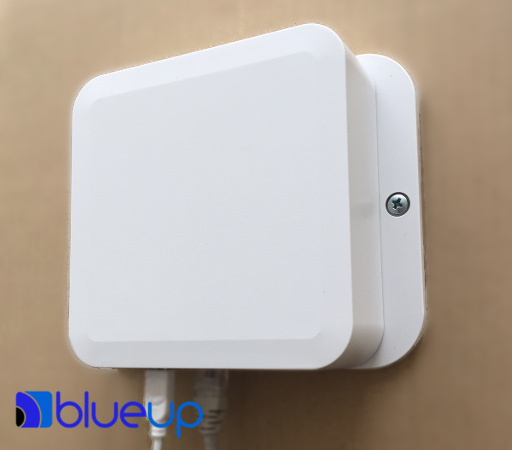
\includegraphics[scale=0.4]{img/cap4/gateway}
\end{figure}

Le principali componenti usate sono:
\begin{itemize}
    \item scheda di rete wireless
    \item chip Bluetooth versione 5
    \item PoE (Power over Ethernet)
\end{itemize}

I gateway forniti dall'azienda BlueUp hanno al loro interno già un firmware che all'avvio del sistema operativo
raspbian avvia il servizio di ranging.
La feature che distingue questi gateway è che sono programmati per chiamare un servizio HTTP custom 
al quale, tramite metodo POST, vengono inviati la lista degli ibeacon in modalità advertising intercettati.

Queste chiamate HTTP, ricevute da un microservizio specializzato di eServant, registrano che nella data
di ricezione sono stati intercettati una serie di ibeacon con una determinata prossimità (BASSA,MEDIA,ALTA).

Visto che i gateway hanno una posizione fissa all'interno dell'impianto, sono stati catalogati nel nostro
database con le coordinate di installazione.
Queste coordinate rappresenteranno la posizione dei dispositivi mobili (in modalità advertising) quando quest'ultimi
vengono intercettati dal gateway attivo.

\subsection{iBeacon passivi}
Gli iBeacon passivi sono un'altro dispositivo standalone dotati di batteria e facilmente maneggevoli per
geolocalizzare un dispositivo all'interno di uno spazio indoor.
Rispetto ai gateway attivi hanno il vantaggio di essere molto più economici (5 volte meno) e di essere
dotati di batterie al litio.

Gli smartphone con eServant installata (in modalità attiva o in background), potranno intercettare
questi dispositivi (come in figura 24) ed inviare tramite HTTP al microservizio specializzato l'ID dell'ibeacon rilevato
per permettere di geolocalizzare il partecipante nelle coordinate dell'ibeacon storicizzate nel nostro
database.

\begin{figure}[H]
    \centering  
    \caption{iBeacon passivi in azione}
    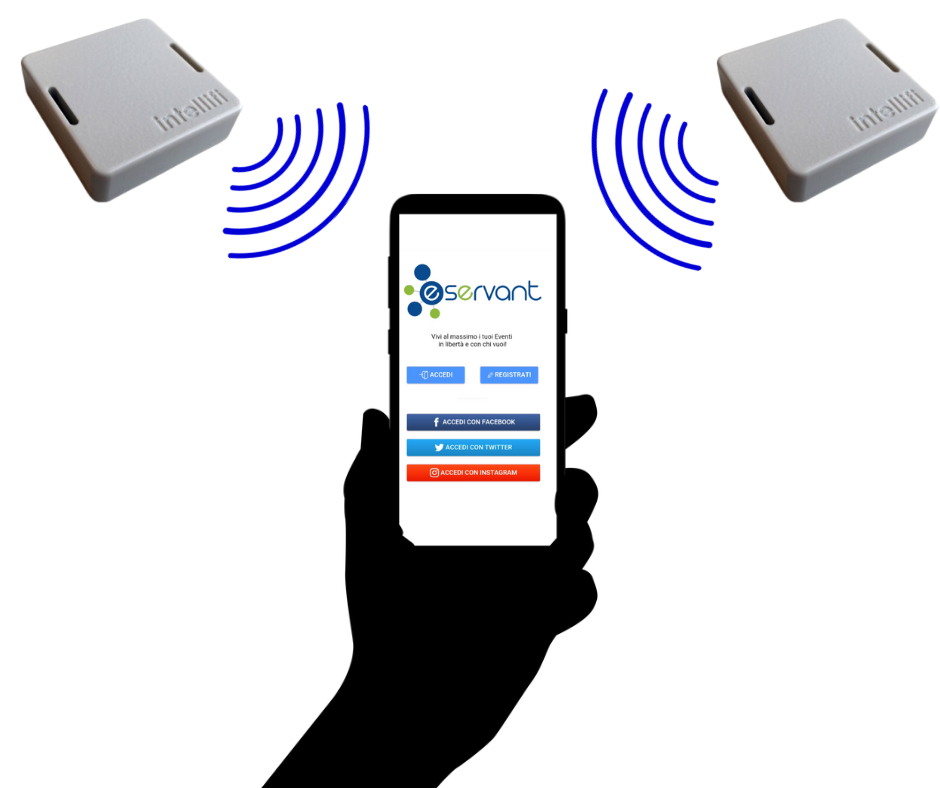
\includegraphics[scale=0.4]{img/cap4/ibeacon-advertising}
\end{figure}

\subsection{iBeacon Wearable}
\begin{figure}[H]
    \centering  
    \caption{iBeacon indossabile}
    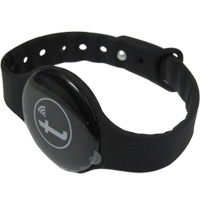
\includegraphics[scale=0.4]{img/cap4/wearable}
\end{figure}
I braccialetti BLE svolgono l'esatto compito degli iBeacon passivi sopra descritti ma vengono utilizzati
con una strategia diversa all'interno di eServant.
Il caso d'uso principale è permettere ai genitori di monitorare real-time la posizione dei propri
figli all'interno di un impianto affollato.
Al genitore, all'ingresso dell'impianto, verranno consegnati un braccialetto (come in figura 25) per ogni figlio.

Nella sezione ricerca un minore dell'app eServant scansionerà il QRcode sopra il braccialetto e da quel momento
in poi il suo utente sarà abilitato a monitorare l'ultima posizione rilevata di ogni singolo braccialetto.
L'assegnazione dei braccialetti viene rilasciata in maniera spontanea all'uscita dall'impianto oppure 
tramite un sistema automatico alcune ore dopo la fine dell'evento (nel caso in cui il genitore non riconsegni
i braccialetti).

I passi sopra descritti sono riportati in figura 26.
\begin{figure}[htp]
    \centering  
    \caption{Caso d'uso braccialetti iBeacon}
    \subfloat[Scanner]{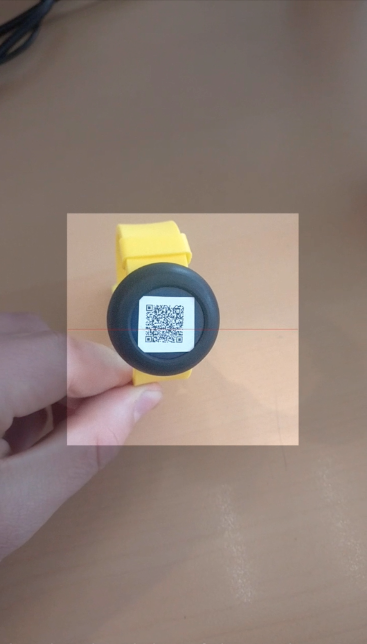
\includegraphics[scale=0.3]{img/cap4/wearable-1}}
    \subfloat[Nome]{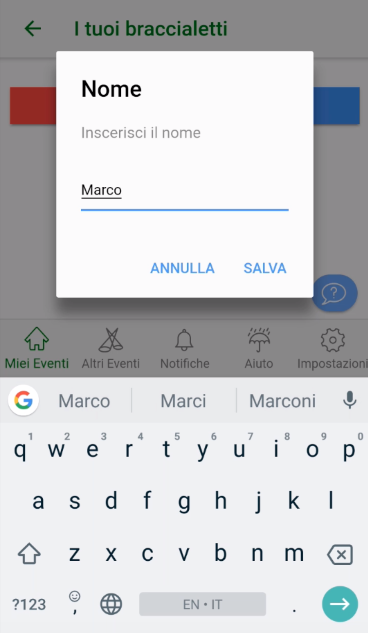
\includegraphics[scale=0.3]{img/cap4/wearable-2}}
    \subfloat[Braccialetti registrati]{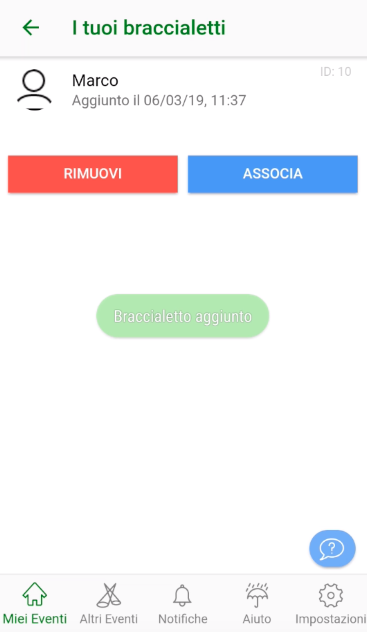
\includegraphics[scale=0.3]{img/cap4/wearable-3}}
    \subfloat[Geolocalizzazione]{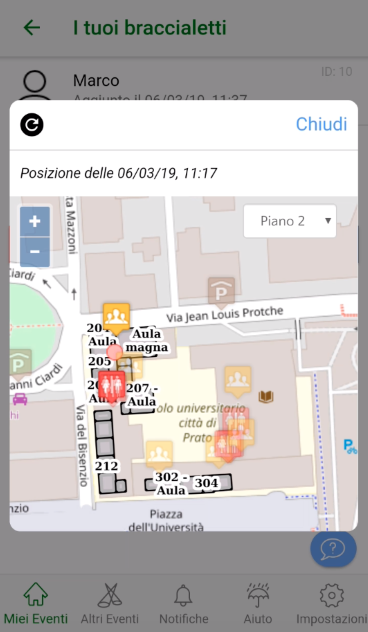
\includegraphics[scale=0.3]{img/cap4/wearable-4}}

\end{figure}

\subsection{Smartphone}
Gli smarthone dei partecipanti agli eventi, tramite l'app di eServant attiva o in background, agiscono
sia in modalità advertising per essere intercettati da eventuali gateway sia in modalità attiva (scanning) per 
intercettare i dispositivi passivi.

\section{Conta persone}

\begin{figure}[H]
    \centering  
    \caption{Single board computer Raspberry}
    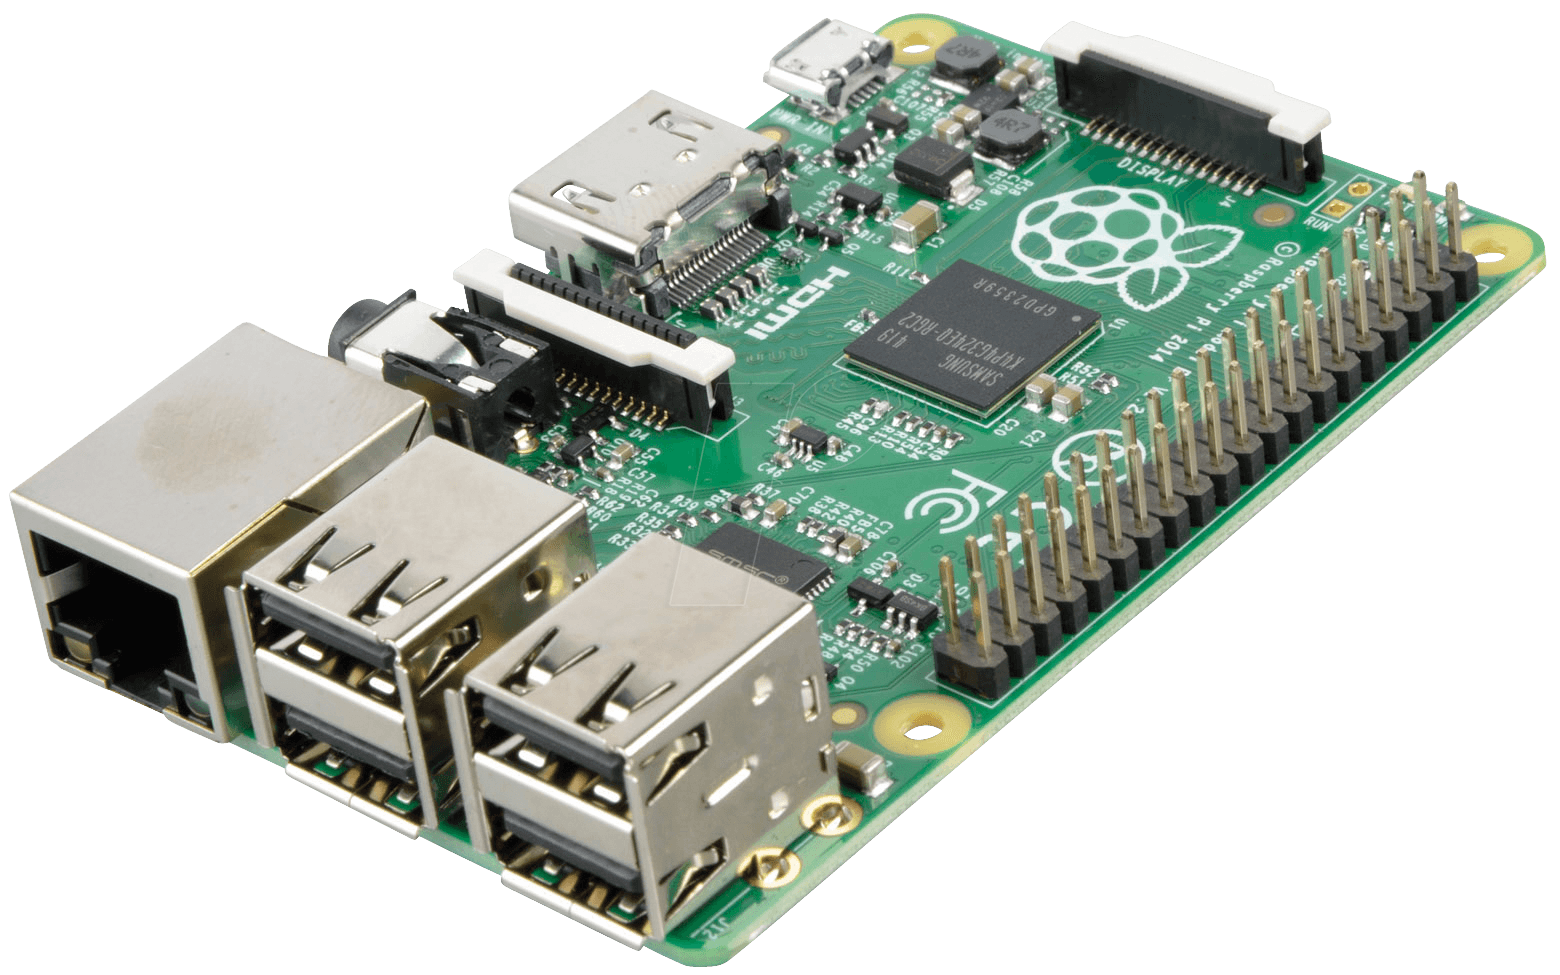
\includegraphics[scale=0.2]{img/cap4/raspberry}
\end{figure}


Il conta persone, come i gateway BLE, è stato implementato sempre usando single board computer
Raspberry.
È dotato inoltre di modulo camera e individua, usando librerie plugAndPlay, le persone che transitano 
dalla porta della biblioteca dove è stato installato.

\begin{figure}[H]
    \centering  
    \caption{Modulo camera per Raspberry}
    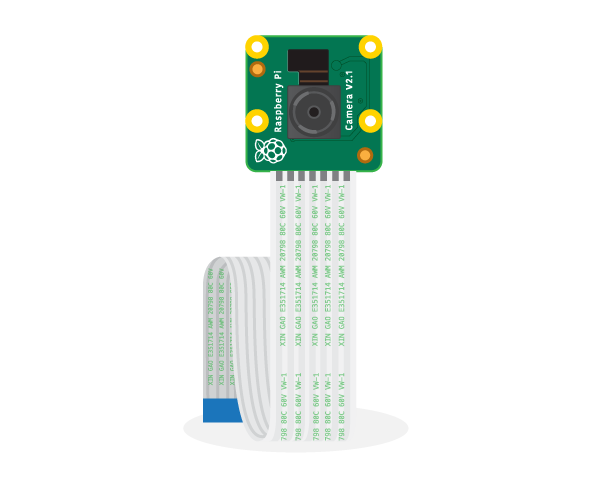
\includegraphics[scale=0.2]{img/cap4/camera}
\end{figure}

Il conta persone mantiene al suo interno un contatore delle persone attualmente dentro l'aula
inviandole con cadenza di 5 minuti ad un microservizio specializzato di eServant che provvede ad
aggiornare il dato sul database.
